\documentclass[a4paper,11pt]{article}

\usepackage{latexsym}
\usepackage[MeX]{polski}
\usepackage{graphicx,caption}
\usepackage{geometry}
\newgeometry{tmargin=1.5cm, bmargin=1.5cm, lmargin=2.0cm, rmargin=2.0cm}
\renewcommand{\refname}{Referencje}
\author{Piotr~Fiborek}
\title{Zastosowanie funkcji identyfikacji uszkodzenia wspomaganej modelowaniem numerycznym do monitorowania stanu technicznego konstrukcji kompozytowych w zmiennych warunkach otoczenia - raport końcowy}
\frenchspacing
\date{}
\begin{document}
	%\maketitle

%\abstract{Głównym celem projektu było stworzenie nowego podejścia do wykrywania uszkodzeń, opierającego się na propagacji fal prowadzonych. Kluczowym elementem proponowanej metody było zrozumienie, jak wielkość uszkodzenie wpływa na charakterystyczne parametry fal sprężystych, które rozchodzą się w badanej konstrukcji. Ze względu na trudność eksperymentalnego uzyskania takich informacji, zdecydowano się na opracowanie modelu numerycznego do symulacji komputerowej.
%W tym celu, stworzono model numeryczny przy użyciu metody spektralnych elementów skończonych w dziedzinie czasu. Model zastosowano do panelu składającego się z rdzenia w postaci plastra miodu z aluminium oraz okładziny z kompozytu wzmocnionego włóknem węglowym. Opracowany model nie tylko jest wydajny obliczeniowo, ale również precyzyjnie odwzorowuje propagację fal w skomplikowanej strukturze.	

%Poprzez przeprowadzenie serii symulacji dla różnych rozmiarów uszkodzenia, przyjętego jako  odklejenie rdzenia od okładziny, opracowano funkcje identyfikacji uszkodzenia (z ang. model-assisted damage identification function, MADIF). W projekcie zbadano również wpływ temperatury otoczenia na MADIF. Porównano uzyskane z symulacji funkcje MADIF z wynikami eksperymentalnymi, które wykazały bardzo dobre dopasowanie pomiędzy modelem a rzeczywistością.
%Dodatkowo przeprowadzono studium parametryczne, w którym określono wpływ różnych parametrów na propagację fal w panelu.

%W rezultacie projektu udało się opracować skuteczne podejście do identyfikacji uszkodzeń poprzez analizę propagacji fal prowadzonych, co ma potencjał w dziedzinie diagnostyki i bezpieczeństwa konstrukcji.

\section{Osiągnięcia}
\subsection{Implementacja interfejsu sprzęgającego elementy o niedopasowanych siatkach w ramach SEM}
W kontekście badania propagacji fal w konstrukcji panelu o rdzeniu w postaci plastra miodu osiągnięto znaczący postęp poprzez wprowadzenie innowacyjnego interfejsu służącego do łączenia komponentów konstrukcyjnych. Interfejs umożliwia skuteczne połączenie elementów, nawet w przypadku, gdy węzły siatek tych komponentów nie pokrywają się geometrycznie. Dotychczas w metodzie spektralnych elementów skończonych (z ang. spectral element method, SEM), konieczne było dopasowanie siatek poprzez generowanie zbieżnych węzłów przylegających elementów. Nowa strategia z interfejsem eliminuje konieczność takiego dostosowywania, otwierając nowe perspektywy w analizie numerycznej.

Zastosowany interfejs bazuje na wykorzystaniu mnożników Lagrange’a jako sił gwarantujących odpowiednie przemieszczenia łączonych elementów, co stanowi znane rozwiązanie w klasycznej metodzie elementów skończonych. Jednakże, aby przenieść siły działające poza węzłami, wykorzystano funkcje kształtu elementów spektralnych.
Wprowadzenie omawianego interfejsu ma istotny wpływ na rozwój SEM. Wcześniej, w sytuacji, gdy zachodziła potrzeba połączenia dwóch elementów znacząco różniących się wymiarami, jak na przykład płyta i czujnik piezoelektryczny (PZT), wymagane było dopasowanie siatek całego modelu, w konsekwencji otrzymywano przewymiarowany model pod względem liczby stopni swobody. Dzięki nowemu podejściu, siatki poszczególnych komponentów generowane są niezależnie, co istotnie usprawnia proces modelowania i analizy. Model z interfejsem znalazł również zastosowanie w symulacji rejestracji fal sprężystych przy wykorzystaniu światłowodowych czujników z siatką Bragga \cite{fiborek2022spectral}.

Wprowadzone innowacje stanowią istotny wkład w dziedzinę analizy strukturalnej za pomocą SEM, otwierając drogę do bardziej efektywnego badania skomplikowanych konstrukcji i przyczyniając się do dalszego postępu w dziedzinie inżynierii.

\subsection{Wyznaczenie MADIF dla panelu przekładkowego}
Przygotowano wysoce efektywny obliczeniowo model numeryczny oparty na SEM \cite{balasubramaniam2021damage, fiborek2021model-assisted} propagacji fal spreżystych w panelu przekładkowym z zachowaniem pełnej geometrii rdzenia typu plaster miodu. W celu potwierdzenia poprawności modelu przeprowadzono szczegółową walidację eksperymentalną, wykorzystując w tym celu wibrometr laserowy oraz zestaw pomiarowy do wzbudzania i rejestracji fal sprężystych przy użyciu czujników piezoelektrycznych (PZT). Również dokonano walidacji modelu samego czujnika poprzez analizę impedancji elektromechanicznej.
Następnie przeprowadzono serię symulacji komputerowych w celu wyznaczenia funkcji identyfikacji uszkodzenia (z ang. model-assisted damage identification function, MADIF) dla przypadku rozklejenia rdzenia od okładziny. W analizie uwzględniono dwa modele uszkodzenia: usunięcie komórek rdzenia oraz usunięcie elementów interfejsu w obszarze rozklejenia. Z sześciu potencjalnych wskaźników uszkodzenia, wybrano dwa, których wartości monotonicznie zmieniały się w miarę wzrostu rozklejenia. Ponadto, wyznaczono MADIF dla modelu rdzenia o jednorodnych właściwościach materiałowych. Porównano obie funkcje z wynikami eksperymentalnymi, co potwierdziło, że proponowany model o pełnej geometrii rdzenia dokładniej odwzorowuje zjawisko propagacji fal sprężystych w panelu przekładkowym.

\subsection{Wyznaczenie MADIF w warunkach zmiennej temperatury otoczenia}
Materiały kompozytowe wykorzystywane są w praktyce w szerokim zakresie temperatur otoczenia, w związku z tym przeprowadzono analizę wpływu zmian warunków zewnętrznych na charakterystykę MADIF. W modelu przyjęto zmiany własności mechanicznych komponentów panelu oraz piezo- i elektromechaniczne parametry czujników.
Wysoka prędkość propagacji fal prowadzonych  (z ang. guided waves, GW) sprawia, że pojedynczy pomiar trwa do 2 ms.
W porównaniu do powolnych zmian temperatury otoczenia (w sekundach), zjawisko propagacji może być modelowane dla stacjonarnego pola temperatury. Założono, że pole temperatury można uzyskać z termometrów w momencie wzbudzenia fali oraz dla uproszczenia w modelu przyjęto jednolite pole temperatury.

\subsection{Studium parametryczne propagacji fal sprężystych w panelu przekładkowym}
Celem przeprowadzonej analizy było dokładne zrozumienie wpływu różnych parametrów geometrycznych i materiałowych komponentów panelu na charakterystyki propagacji fal prowadzonych w tej konstrukcji. W szczególności, badanie skupiło się na analizie zmian amplitudy oraz prędkości grupowej pierwszych paczek modułów S0 i A0.

W ramach badania wzięto pod uwagę szeroki zakres kluczowych parametrów, mających wpływ na zjawisko propagacji fal w badanym panelu. Wśród analizowanych parametrów znalazły się: piezo- i elektromechaniczne właściwości czujników oraz dokładne położenie czujników piezoelektrycznych względem komórki plastra miodu, a także właściwości materiałów wykorzystanych do okładziny oraz warstwy kleju. Dodatkowo, uwzględniono geometryczne parametry rdzenia konstrukcji oraz różne warunki brzegowe, które mogą wpływać na charakter propagujacych się fal.

Powyższe parametry można podzielić na dwie kluczowe kategorie: te, które pozostają stałe w trakcie analizowanego okresu, oraz te, które mogą ulegać zmianom pod wpływem warunków otoczenia lub w wyniku procesów starzenia się komponentów konstrukcji. Parametry z pierwszej grupy obejmują między innymi wymiary geometryczne rdzenia, udział włókien węglowych w materiale oraz precyzyjne rozmieszczenie czujników względem komórki plastra miodu. W drugiej grupie znajdują się zaś parametry materiałowe komponentów.
Warto podkreślić, że parametry z pierwszej grupy pozostają niezmienne zarówno w przypadku stanu referencyjnego, jak i w trakcie monitorowania konstrukcji, które nie będą wpływać na przebieg MADIF w czasie.

W kontekście praktycznego wykorzystania zaproponowanej metody, istotnym krokiem jest opracowanie skutecznego narzędzia do identyfikacji parametrów z drugiej grupy. Tylko wtedy możliwa będzie precyzyjna kalibracja modelu numerycznego, co stanowi kluczowy element dla pomyślnego wdrożenia tej metody w praktyce.

Dokładna analiza tych parametrów daje solidną podstawę do zrozumienia zachowania struktury w odpowiedzi na propagujące fale sprężyste oraz do opracowania skutecznych strategii monitorowania i diagnozowania ewentualnych zmian w konstrukcji.

\subsection{Złożenie dysertacji}
W ramach projektu przeprowadzone badania pozwoliły autorowi napisać rozprawę doktorską zatytułowaną "Modelling of Sandwich Plates and Piezoelectric Transducers for the Identification of Mechanical Damage Severity" \cite{fiborek2023modelling}. 
Dysertacja została złożona do Rady Naukowej IMP PAN i otrzymała dwie pozytywne recenzje, niezbędne w celu przystapienia do publicznej obrony rozprawy doktorskiej.

\section{Uzyskane wyniki badań}
W ramach projektu zamodelowano panel przekładkowy z zachowaniem pełnej geometrii rdzenia typu plaster miodu (z ang. full core geometry model, FCGM). Taki model okazał się bardziej adekwatny w odwzorowaniu rzeczywistej propagacji fal sprężystych w konstrukcji, niż model, w którym parametry materiałowe rdzenia były homogenizowane (z ang. homogenised core geometry model, HCGM). Na Rysunku~\ref{fig:fullfield} zaprezentowano wybrane momenty propagacji fal sprężystych obu modeli w zestawieniu z pomiarami dokonanymi za pomocą wibrometru laserowego. W proponowanym modelu doskonale widoczne są interakcje fal w komórkach rdzenia, podobnie jak w pomiarach eksperymentalnych. W przypadku uproszczonego modelu, obserwuje się płynną propagację fali, co wpływa na mniejszą dokładność wskaźnika MADIF.

\begin{figure}[ht]
	\centering
	\captionsetup{width=.9\textwidth}
	\includegraphics[width=0.6\textwidth]{fullfield_100_0}
	\caption{Porównanie propagacji fal sprężystych w modelach FCGM i HGCM oraz wyników~eksperymentalnych.}
	\label{fig:fullfield}
\end{figure}

W wyniku przeprowadzonych symulacji komputerowych, wydzielono sześć wskaźników uszkodzenia, z których dwa, a mianowicie odchylenie pierwiastka średniej kwadratowej (RMSD) oraz współczynnik korelacji Pearsona (CC), wykazywały monotoniczny spadek wartości wraz ze zwiększającym się stopniem uszkodzenia. Obie te miary dokładnie korelują z funkcjami uzyskanymi eksperymentalnie (z ang. experimental damage identification function, EDIF), co można zaobserwować na Rysunku~\ref{fig:madif}.

\begin{figure}[hb]
	\centering
	\captionsetup{width=.9\textwidth}
	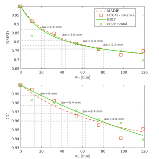
\includegraphics[width=0.9\textwidth]{MADIF_20}
	\caption{Porównanie MADIF oraz eksperymentalnej funkcji identyfikacji uszkodzenia (EDIF) opartych na RMSD i CC.}
	\label{fig:madif}
\end{figure}

Podobnie, w analizie zmiennych temperatur otoczenia, wskaźnik MADIF wykazywał zgodność z wynikami uzyskanymi eksperymentalnie, szczególnie w zakresie temperatur od \(+10^\circ\)C do \(+50^\circ\)C (Rysunek~\ref{fig:madif_temp_RMSD}). Niemniej jednak, dla temperatur poniżej \(0^\circ\)C wartości MADIF znacząco odbiegały od EDIF, co sugeruje, że liniowy model właściwości materiałowych komponentów w funkcji temperatury otoczenia nie jest dostatecznie precyzyjny w odniesieniu do rzeczywistego obiektu.

Rysunek \ref{fig:pzt_place} ukazuje wyniki studium parametrycznego, prezentując sygnały zarejestrowane dla różnych lokalizacji czujników względem komórki plastra miodu, przy czym odległość między wzbudzeniem a rejestrowaniem sygnału jest stała.

\begin{figure}
	\centering
	\captionsetup{width=.9\textwidth}
	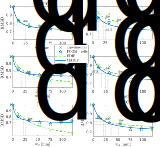
\includegraphics[width=0.75\textwidth]{MADIF_temp_RMSD}
	\caption{Porównanie MADIF oraz funkcji identyfikacji uszkodzenia (EDIF) opartych na RMSD i CC w zależności od temperatury otoczenia.}
	\label{fig:madif_temp_RMSD}
\end{figure}
\begin{figure}
	\centering
	\captionsetup{width=.9\textwidth}
	\includegraphics[width=0.75\textwidth]{pzt_place}
	\caption{Propagacja fal sprężystych w panelu przekładkowym (\textbf{a}), zarejestrowane sygnały dla (\textbf{b}) różnej lokalizacji czujników względem komórek plastra miodu.}
	\label{fig:pzt_place}
\end{figure}
W związku z ograniczeniami przestrzennymi niniejszego raportu, wybrane zostały tylko niektóre wyniki badań.
Pozostałe wyniki badań i analiz, zostały zaprezentowane podczas konferencji naukowych \cite{fiborek2023model, fiborek2023parametric}, a także opublikowane w czasopismach naukowych \cite{balasubramaniam2021damage, balasubramaniam2021ultrasonic, balasbramaniam20021experimental, balasubramaniam2021lamb} oraz rozprawie doktorskiej \cite{fiborek2023modelling}. 

Najważniejsze wnioski wynikające z badań i otrzymanych wyników to:
\begin{itemize}
	\item model z pełną geometrią plastra miodu w porównaniu do modelu homogenizowanego jest dokładniejszy,
	\item temperatura otoczenia ma silny wpływ na wskaźnik MADIF,
	\item zjawisko propagacji fali sprężystej w panelu jest bardzo złożone, a wartość amplitudy i prędkość fali silnie zależą od wielu parametrów poszczególnych komponentów, wzbudzenia sygnału i warunków środowiskowych,
	\item konieczne jest opracowanie metody identyfikacji parametrów materiałowych i geometrycznych struktury, aby umożliwić adekwatną kalibrację modelu.
\end{itemize}

\section{Realizowane cele}
W procesie realizacji głównego celu projektu, którym było opracowanie funkcji identyfikacji wielkości uszkodzenia w panelu przekładkowym w zmiennych warunkach otoczenia, zostały osiągnięte znaczące kroki w dziedzinie analizy struktur i diagnostyki uszkodzeń mechanicznych. Wykazano, że modelowanie panelu z pełną geometrią rdzenia plastra miodu przynosi dokładniejsze wyniki w odniesieniu do propagacji fal sprężystych niż uproszczony model homogenizacji materiałów. Dokładna analiza parametrów struktury, zapewniła solidną podstawę do lepszego zrozumienia złożonego zjawiska propagacji fal sprężystych w panelu przekładkowym.

\section{Wpływ na dyscyplinę naukową}
Zaproponowane strategie diagnozowania ewentualnych zmian w konstrukcji, oparte na opracowanym modelu numerycznym, mają potencjał przełożenia się na praktyczne zastosowanie w metodach monitorowania stanu technicznego konstrukcji.
Ponadto, zaimplementowano interfejs dla niepasujących siatek zastosowanych komponentów w ramach metody elementów spektralnych w dziedzinie czasu, co stanowi istotny wkład w rozwój tej metody numerycznej.

\begin{thebibliography}{99}
\bibitem{fiborek2022spectral} \underline{Fiborek,~P.}; Soman,~R.; Kudela,~P.; 		Ostachowicz,~W. Spectral element modeling of ultrasonic guided wave propagation in optical fibers. \textit{Ultrasonics} \textbf{2022}, 124, 106746. doi: 10.1016/j.ultras.2022.106746
\bibitem{balasubramaniam2021damage} Balasubramaniam,~K.; \underline{Fiborek,~P.}; 	Sikdar,~S.; Malinowski,~P. Damage Assessment for a Sandwich-Like Panel Using Experimental and Numerical Analysis of Guided Waves. In: Mukhopadhyay, C.K., Mulaveesala, R. (eds) Advances in Non-destructive Evaluation. Lecture Notes in Mechanical Engineering. Springer, Singapore. \textbf{2021} doi: 10.1007/978-981-16-0186-6\_8
\bibitem{fiborek2021model-assisted} \underline{Fiborek,~P.}; Kudela,~P. Model-Assisted 	Guided-Wave-Based Approach for Disbond	Detection and Size Estimation in Honeycomb Sandwich Structures. \textit{Sensors} \textbf{2021}, 21, 8183. doi: 10.3390/s21248183
\bibitem{fiborek2023modelling} \underline{Fiborek,~P.} Modelling of Sandwich Plates and Piezoelectric Transducers for the Identification of Mechanical Damage Severity. Rozprawa doktorska, IMP PAN Gdańsk, \textbf{2023}
\bibitem{fiborek2023model} \underline{Fiborek,~P.}, Kudela,~P. Model-assisted method for damage severity assessment in honeycomb sandwich panel. NDT in Canada 6-8 June \textbf{2023}, Edmonton Canada
\bibitem{fiborek2023parametric} \underline{Fiborek,~P.}, Kudela,~P. Parametric study of guided wave propagation in honeycomb sandwich panel for model-assisted damage assessment method. \(7^{th}\) International Conference of Engineering Against Failure, 21-23 June \textbf{2023}, Spetses Greece
\bibitem{balasubramaniam2021ultrasonic} Balasubramaniam,~K.; Sikdar,~S.; \underline{Fiborek,~P.}; Malinowski,~P. Ultrasonic Guided Wave Signal Based Nondestructive Testing of a Bonded Composite Structure Using Piezoelectric Transducers \textit{Signals}. \textbf{2021}, 2, 13-24. doi: 10.3390/signals2010002
\bibitem{balasbramaniam20021experimental} Balasubramaniam,~K.; Ziaja,~D.; Jurek,~M.; \underline{Fiborek,~P.}; Malinowski,~P. Experimental and Numerical Analysis of Multiple	Low-Velocity Impact Damages in a Glass Fibered Composite Structure. \textit{Materials} \textbf{2021}, 14, 7268. doi: 10.3390/ma14237268
\bibitem{balasubramaniam2021lamb} Balasubramaniam,~K.; \underline{Fiborek,~P.}; Malinowski,~P. Lamb waves based assessment of impact damage in multilayered CFRP plate. Proc. SPIE 11593, Health Monitoring of Structural and Biological Systems XV, 115930O (22 March \textbf{2021}). doi: 10.1117/12.2583950
\end{thebibliography}
\end{document}